% !TEX TS-program = pdflatexmk
\documentclass[12pt]{article}

\usepackage{amsthm}

% Layout.
\usepackage[top=.75in, bottom=0.75in, left=.75in, right=.75in, headheight=1in, headsep=6pt]{geometry}

% Fonts.
\usepackage{mathptmx}
\usepackage[scaled=0.86]{helvet}
\renewcommand{\emph}[1]{\textsf{\textbf{#1}}}

% Misc packages.
\usepackage{amsmath,amssymb,latexsym}
\usepackage{graphicx,tikz}
\usepackage{array}
\usepackage{xcolor}
\usepackage{multicol}
\usepackage{tabularx,colortbl}
\usepackage{enumitem}
%to make tikz pics work
\usepackage{tikz,pgfplots}
\usetikzlibrary{arrows}
\newcommand{\midarrow}{\tikz \draw[-triangle 90] (0,0) -- +(.1,0);}

\usepackage[colorlinks=true]{hyperref}

% Paragraph spacing
\parindent 0pt
\parskip 6pt plus 1pt
\def\tableindent{\hskip 0.5 in}
\def\ts{\hskip 1.5 em}

\usepackage{fancyhdr}
\pagestyle{fancy} 
\lhead{\large\sf\textbf{MATH 663 }}
\rhead{\large\sf\textbf{Fall 2023}}
\chead{\large\sf\textbf{HW 4}}

\newcommand{\localhead}[1]{\par\smallskip\textbf{#1}\nobreak\\}%
\def\heading#1{\localhead{\large\emph{#1}}}
\def\subheading#1{\localhead{\emph{#1}}}

%% Special Math Symbol shortcuts
\newcommand{\bbN}{\mathbb{N}}
\newcommand{\rad}{\text{rad}}
\newcommand{\diam}{\text{diam}}
\newcommand\solution{\localhead{Solution:}}

%\newenvironment{clist}%
%{\bgroup\parskip 0pt\begin{list}{$\bullet$}{\partopsep 4pt\topsep 0pt\itemsep -2pt}}%
%{\end{list}\egroup}%

\usetikzlibrary{calc,arrows.meta}
%\pgfplotsset{my style/.append style={axis x line=middle, axis y line=
%middle, xlabel={$x$}, ylabel={$y$}, axis equal }}


\begin{document}
\begin{enumerate}

	\item Go back and re-read your proof for problem 1 on Homework \# 2. Go back and read Jill's proof of the same problem. (In some cases, Jill's solution may be the same as yours. In some cases, you may want to re-think your original proof.) For this problem, either copy or re-write your original proof into your homework. Then, answer the questions, ``What did I \emph{actually} prove? What did Jill actually prove?" That is, in every case, the proofs established a \emph{stronger} result than the problem stated.
	

	\begin{proof}
		\textbf{Stefano's Proof:} Let $G$ be a 2-connected graph and consider vertex $x$. Note that since $G$ is 2-connected, $x$ must have at least two neighbors $y$ and $z$, otherwise, the removal of the single neighbor would disconnect $x$ from the graph. Note $G - x$ is connected, so let $yPz$ be the path in $G - x$. Clearly we can form a cycle with $yPz$ and $x$. 
	\end{proof}



	\begin{proof}
		\textbf{Jill's Proof:}  Suppose that $G$ is a 2-connected graph. Then, by definition, $G$ is connected and has at least 3 vertices. Let $e=uv$ be an edge of $G$. Since $G$ is 2-connected, $2 \leq \kappa(G) \leq \lambda(G).$ Now, by the definition of edge-connectivity, $G-e$ is connected. Thus, there exists a $uv$-path in $G-e.$ This $uv$-path along with edge $e$ forms a cycle in $G.$\\
	\end{proof}

	I am not certain at what you are getting at with this question. It feels as though both proofs are correct in solving the problem, albeit yours manages do it by removing an edge from the graph and mine manages by removing a vertex. 

	I think maybe the stronger result that is proven is that $\emph{every}$ edge(from yours) and vertex(mine) lies on some cycle in a 2-connected graph.
	\newpage



	\item Prove that if $G$ is a graph (not necessarily a bipartite graph) with matching $M$ and vertex cover $U,$ then $|M|\leq |U|$.
	\begin{proof}  Let $G$ be a graph with $M$ a matching and $U$ a vertex cover. By definition the vertices of $U$, "cover" the edges of $G$ i.e. the vertices $U$ are incident to all $E(G)$ and therefore all of $M$. It must then follow that there can never be more than 1 edge from $M$ incident to a vertex of $U$, 
		otherwise $M$ would contain two edges incident to the same vertex and would no longer be a matching. 
		Therefore at best, meaning every vertex in $U$ is actually incident to an edge in $M$, there is a bijective map between $U$ and $M$ but otherwise it must be surjective. Hence $|M|\leq |U|$. 





	\end{proof}
	\newpage



	\item Read and understand the second proof of Hall's Theorem in our text. Then, write up a \emph{complete} proof, with all the details, in your own words. 
	\begin{proof} Let $G$ be a bipartite graph, with bipartite sets $A$ and $B$. Suppose $G$ satisfies $|N(S)| \geq |S|$ for all $S \subseteq A$. We will proceed to show that $G$ contains a matching which saturates $A$ via induction on $|A|$.  

		For the base case we consider $|A| = 1$, since the graph $G$ is bipartite either $G$ has no edges, in which case $M = \emptyset$. Alternately, since $|N(A)| \geq |A| = 1$, choosing a single $e \in N(A)$ is sufficient for a matching which saturates $A$.\\


		Let $|A| = n$ and suppose our graph $G$ satisfies a stronger version of the hypothesis $|N(S)| \geq |S| + 1$ for every non-empty set $S \subseteq A$. Consider an edge $ab \in G$ then define $G' := G - \{a, b\}$. Let $A' = A \setminus \{a\}$ and $S \subseteq A'$ and note that either $b \in N_G(S)$ in which case $|N_G'(S)| = |N_G(S)| - 1$ or $b \not\in N_G(S)$ in which case $|N_G'(S)| = |N_G(S)| > |N_G(S)| - 1$. Hence 
		\begin{equation*}
			|N_G'(S)| \geq |N_G(S)| - 1 \geq |S|. 
		\end{equation*} 
		Since $|A'| = n - 1$ by the induction hypotheses $G'$ contains a matching $M'$, which saturates $A'$.
		Clearly $M = M' \cup \{ab\}$ will now saturate $A$ in $G$. \\

		
		
		Now suppose our graph $G$ does \emph{not} satisfy the stronger hypothesis, so there exists a nonempty $A' \subset A$ (Note $A'$ must be a proper subset since assuming otherwise finding a matching set which saturates $A$ would be trivial) such that $|N(A')| = |A'|$. 
		
		Note that $G':=G[A' \cup B']$ has $|A'| < n$ and is an induced subgraph of $A$, so it must satisfy Hall's Condition and therefore contains a matching $M_1$, which saturates $A'$. 
		
		
		Suppose to the contrary that $G - G'$ fails to satisfy Hall's Condition. There exists $S \subseteq A \setminus A'$ such that $|N_{G - G'}(S)| < |S|$. Then $S \cup A'$ would be a subset in $G$ which fail Hall's Condition, a contradiction. 
		
		Therefore there exists a matching $M_2$, in $G - G'$ which saturates $A \setminus A'$. Note that $M = M_1 \cup M_2$ is a matching for $G$. 

	\end{proof}
	\newpage



	\item Two players jointly construct a path is a fixed graph $G$ by alternately picking vertices from $G$. If $v_1,v_2,\cdots, v_k$ is the path constructed thus far, the player to move next must find a vertex $v_{k+1}$ such that $v_1,v_2,\cdots, v_k, v_{k+1}$ is also a path in $G.$ A player wins if the opponent has no available move. Prove that the player who goes second has a winning strategy if and only of $G$ contains a 1-factor.

	\begin{proof} Suppose that the game is played on a graph $G$ that contains a perfect matching $M$. Since $G$ contains a perfect matching every vertex is saturated and therefore Player 1 must pick a saturated vertex. Since $M$ is a perfect matching, every vertex is incident to exactly edge in $M$. It must be the case that Player 2 can select a vertex such that the edge that is added to the path is an edge from $M$. If Player 2 does so, Player 1 will only be able to pick a vertex such that the edge that is added to the path is not from $M$. Since $M$ is a matching it contains no augmenting paths, and since $M$ spans the graph, every path produced by this game must end in an unmatched edge which means Player 2 had the last vertex.
	\end{proof}
		

   
   
   \begin{proof}
	Suppose that the game is played on a graph $G$ that does not contain a perfect matching. Let $M$ be a maximum matching. Suppose that Player 1 selects an unsaturated vertex. From here it follows that whichever vertex Player 2 selects it must be saturated by $M$ otherwise the edge, $e$ that is added to the path would be incident to two unsaturated vertices and would therefore make $M + e$ the maximum matching. 
	
	Now Player 1 will have the option to choose a vertex which adds an edge from $M$, otherwise if no such vertex exists and the game was $\emph{not}$ over, the path that would result would be an augmenting path, contradicting $M$ being the maximum matching. Hence Player 1 is guaranteed to win and there Player 2 has no winning strategy. 
	\end{proof} 
   





	\newpage



	\begin{enumerate}
	\item Let $A_1 =\{a,b,d\},\: A_2=\{a,b\}, \: A_3=\{a,d\}$, and $A_4=\{a,c\}$ by subsets of the set $A=\{a,b,c,d\}.$ Show that for every integer $i$, $1 \leq i \leq 4,$ there exists $x_i \in A_i$ such that $x_i \not = x_j$ if $i \not = j.$ The set $S=\{x_1,x_2,x_3,x_4\}$ is called a \emph{system of distinct representatives} for the subsets $A_i.$ (No proof needed here. Just find the system of distinct representatives.)
	\solution Consider the following, 
	\begin{equation*}
		S = \{a_1, b_2, d_3, c_4\}
	\end{equation*}
	\begin{equation*}
		S = \{b_1, a_2, d_3, c_4\}
	\end{equation*}


	\item Let $A$ be a finite set with subsets $A_1, A_2, \cdots, A_k.$ Prove that there exists a system of distinct representatives of the family of sets $A_1, A_2, \cdots, A_k$ if and only if for every $I\subseteq\{1,2,\cdots,k\},$ $\displaystyle{\left\vert \cup_{i \in I} A_i\right\vert \geq |I|.}$
	\end{enumerate}
	\begin{proof} Let $A$ be a finite set with subsets $A_1, A_2, \cdots, A_k$, $K= [k]$ and
		Let $G$ be a bipartite graph between partite sets $A$ and $K = [k]$ defined by the symmetric relation $g: A \to K$ such that $a \sim i$ if $a \in A_i$. 
		
		$\rightarrow$ Suppose there exists a system of distinct representatives defined by the set $S$. The relation $g$ restricted to $S$ will then become a bijective function which represents a matching of $G$ that saturates $K$. So $g|_S$ is well defined since a single representative is chosen for each subset, injective by definition of the set $S$ and therefore must be surjective since $|S| = |K|$. Since $G$ has a matching which saturates $K$, by Hall's Theorem we conclude that for every $I\subseteq K$, it follows that $\displaystyle{\left\vert \cup_{i \in I} A_i\right\vert \geq |I|.}$
		
		

		$\leftarrow$ Suppose that for every $I\subseteq\{1,2,\cdots,k\}$, it follows that $\displaystyle{\left\vert \cup_{i \in I} A_i\right\vert \geq |I|}$. By Hall's Theorem there exists a matching $M$ which saturates $K$. Let $S \subset A$ which are incident to $M$ and consider the restriction $g|_S$. Since $M$ is a matching $g|_S$ is well defined and injective since no two matched edges can be incident to each other. Note that since $M$ saturates $K$, so $g|_s$ is surjective. Therefore by the construction of $g$, $S$ must have a representative from every $A_i$ and by virtue of $g|_S$ being a well-defined injection, $S$ is a system of distinct representatives. 
	\end{proof}
	I acknowledge that this went against the grain a little bit... 


	\newpage







	\item This problem will require you to do two things: (i) go through the argument in Corollary 2.1.5 in a concrete way and (ii) use some TikZ.\\
	Let $G$ be the 4-regular graph on the left below with Eulerian tour: $T=av_0v_1av_2v_1bv_0v_3bv_2v_3a.$\\
	
%%%Table to arrange graphs
\begin{tabular}{cc}
	%%%BEGIN Graph G
	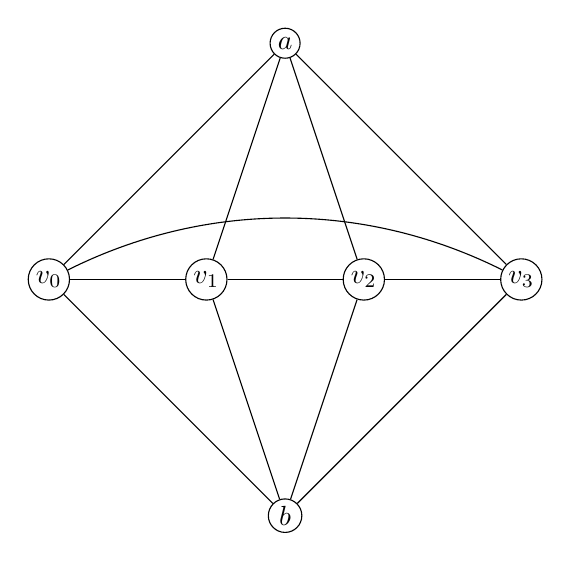
\begin{tikzpicture}[scale=1,every node/.style={draw,circle, inner sep=.05 cm}]
	%top and bottom vertices placed by hand
	\node (a) at (3,3){$a$};\node (b) at (3,-3){$b$}; 
	%%middle vertices drawn with a loop
	%% vertical edges drawn with a loop
	\foreach \i in {0,1,2,3}{
		\node  (\i) at (2*\i,0){$v_{\i}$};
		\draw (a) -- (\i) -- (b);
		}
	%% draw straight edges around the middle
	\draw (0)--(1)--(2)--(3);
	\draw (0) .. controls (2,1) and (4,1) .. (3);
	\end{tikzpicture}
	%%%END Graph G
	&
	%%%BEGIN Euler Tour
	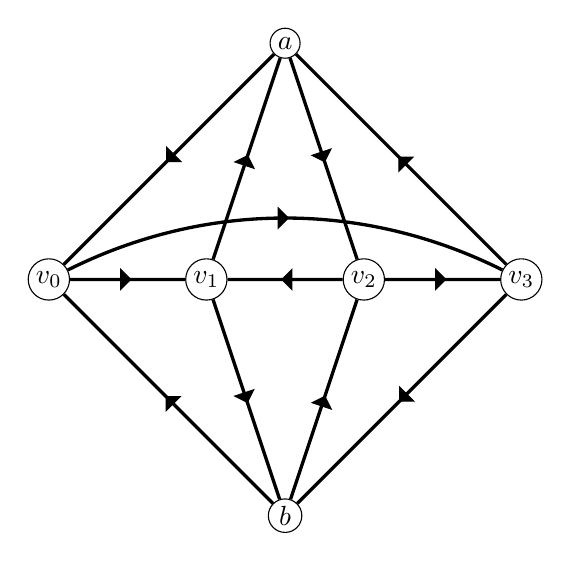
\begin{tikzpicture}[scale=1,every node/.style={draw,circle, inner sep=.05 cm}, every edge/.style = {draw, to reversed-to}]
	%top and bottom vertices placed by hand
	\node (a) at (3,3){$a$};\node (b) at (3,-3){$b$}; 
	%%middle vertices drawn with a loop
	\foreach \i in {0,1,2,3}{
		\node  (\i) at (2*\i,0){$v_{\i}$};
		}
	%% draw euler tour
	\begin{scope}[very thick, every node/.style={sloped,allow upside down}]
	 \draw (a) -- node {\midarrow}(0)-- node {\midarrow} (1) -- node {\midarrow} (a) -- node {\midarrow}(2)-- node {\midarrow}(1)-- node {\midarrow}(b)-- node {\midarrow}(0) (3)-- node {\midarrow}(b)-- node {\midarrow}(2)-- node {\midarrow}(3)-- node {\midarrow}(a);
	\draw (0)  .. controls (2,1) and (4,1) ..  node {\midarrow}(3);
	\end{scope}
	\end{tikzpicture}
	%%%End Euler Tour
	\end{tabular}
	%%%End tablular environment
		\begin{enumerate}
		\item Find two nonisomorphic 2-factors in $G.$ Draw them using TikZ.
		\begin{proof} The following are two nonisomorphic 2-factors of $G$. Note that one subgraph is a single component and the other is two, so it is evident that they are nonisomorphic. \\
		


			\begin{tabular}{cc}
			\begin{tikzpicture}[scale=1,every node/.style={draw,circle, inner sep=.05 cm}]
				%top and bottom vertices placed by hand
				\node (a) at (3,3){$a$};\node (b) at (3,-3){$b$}; 
				%%middle vertices drawn with a loop
				%% vertical edges drawn with a loop
				\foreach \i in {0,1,2,3}{
					\node  (\i) at (2*\i,0){$v_{\i}$};
					}
				%% draw straight edges around the middle
				\draw (1)--(2)--(3);
				\draw (a)--(0);
				\draw (0)--(b)--(3);
				\draw (1)--(a);
				%\draw (0) .. controls (2,1) and (4,1) .. (3);
				\end{tikzpicture}
				&\qquad
				\begin{tikzpicture}[scale=1,every node/.style={draw,circle, inner sep=.05 cm}]
					%top and bottom vertices placed by hand
					\node (a) at (3,3){$a$};\node (b) at (3,-3){$b$}; 
					%%middle vertices drawn with a loop
					%% vertical edges drawn with a loop
					\foreach \i in {0,1,2,3}{
						\node  (\i) at (2*\i,0){$v_{\i}$};
						}
					\draw (a)--(0)--(1)--(a);
					\draw (b)--(2)--(3)--(b);
					%% draw straight edges around the middle
					\end{tikzpicture}
				\end{tabular}
		\end{proof}
		



		\item Define a new graph $H$ with vertex set $V=\{a^+,a^-,b^+,b^-,v_0^+,v_0^-,v_1^+,v_1^-,v_2^+,v_2^-,v_3^+,v_3^-\}$ and edge set $E=\{ x^-y^+ \: \vert \: xy \in E(T) \text{ in that order }\}.$ Draw $H$ in TikZ.
		\begin{proof} This was so difficult for some reason. 
			\begin{center}
			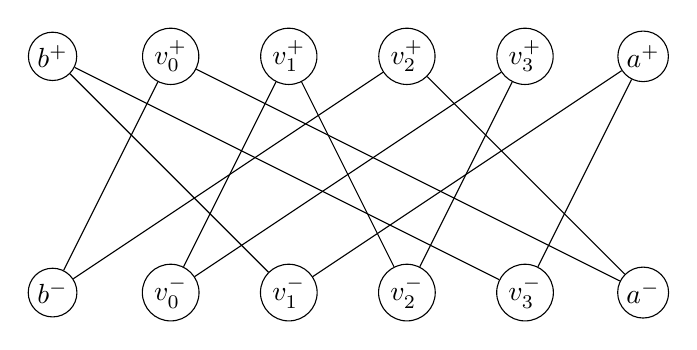
\begin{tikzpicture}[scale=1,every node/.style={draw,circle, inner sep=.05 cm}]
				%top and bottom vertices placed by hand
				%%middle vertices drawn with a loop
				%% vertical edges drawn with a loop
				\node (am) at (1.5*4, 1){${a}^-$};
				\node (ap) at (1.5*4, 4){${a}^+$};
				\foreach \i in {3, 2, 1, 0}{
					\node  (\i-) at (1.5*\i, 1){$v_{\i}^-$};
					\node  (\i+) at (1.5*\i, 4){$v_{\i}^+$};
					}
				\node (bm) at (1.5*-1, 1){${b}^-$};
				\node (bp) at (1.5*-1, 4){${b}^+$};

				\draw (am)--(0+);
				\draw (0-)--(1+);
				\draw (1-)--(ap);
				\draw (am)--(2+);
				\draw (2-)--(1+);
				\draw (1-)--(bp);
				\draw (bm)--(0+);
				\draw (0-)--(3+);
				\draw (3-)--(bp);
				\draw (bm)--(2+);
				\draw (2-)--(3+);
				\draw (3-)--(ap);
 				%\draw (0) .. controls (2,1) and (4,1) .. (3);
				\end{tikzpicture}
			\end{center}
		\end{proof}
		








		\item Explain why $H$ must (i) be bipartite and (ii) satisfy Hall's condition.
		\begin{proof} It is clear that $H$ must be bipartite by the definition $E$, there simply cannot exists an edge between vertices in the positive and negative partite sets. 

			Since the original graph was $2(2)-regular$ every vertex in $T$ has two in-flow edges and two out-flow edges which contribute 2 degrees to each $v^+$ and $v^-$ respectively. Hence the $H$ is 2 regular, and therefore satisfies Hall's condition. 

			
		\end{proof}




		\item Find a 1-factor in $H$.
		
		\begin{proof} A 1-factor of $H$ is highlighted in red below, 
			\begin{center}
			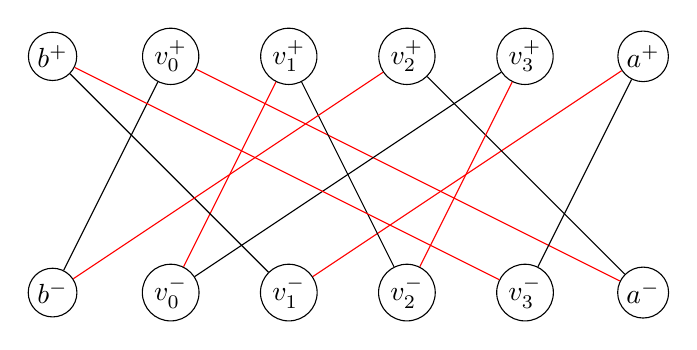
\begin{tikzpicture}[scale=1,every node/.style={draw,circle, inner sep=.05 cm}]
				%top and bottom vertices placed by hand
				%%middle vertices drawn with a loop
				%% vertical edges drawn with a loop
				\node (am) at (1.5*4, 1){${a}^-$};
				\node (ap) at (1.5*4, 4){${a}^+$};
				\foreach \i in {3, 2, 1, 0}{
					\node  (\i-) at (1.5*\i, 1){$v_{\i}^-$};
					\node  (\i+) at (1.5*\i, 4){$v_{\i}^+$};
					}
				\node (bm) at (1.5*-1, 1){${b}^-$};
				\node (bp) at (1.5*-1, 4){${b}^+$};

				\draw [color = red]--(am)--(0+);
				\draw [color = red](0-)--(1+);
				\draw [color = red](1-)--(ap);
				\draw (am)--(2+);
				\draw (2-)--(1+);
				\draw (1-)--(bp);
				\draw (bm)--(0+);
				\draw (0-)--(3+);
				\draw [color = red](3-)--(bp);
				\draw [color = red](bm)--(2+);
				\draw [color = red](2-)--(3+);
				\draw (3-)--(ap);
 				%\draw (0) .. controls (2,1) and (4,1) .. (3);
				\end{tikzpicture}
			\end{center}
		\end{proof}
		







		\item Use the 1-factor in $H$ to find a 2-factor in $G.$ (For this problem it is sufficient to state the 1-factor and then state the 2-factor.)

		\begin{proof} Highlighted in red is a 2-factor for graph $G$ constructed by collapsing the previous 1-factor for graph $H$. 
			\begin{center}
			
			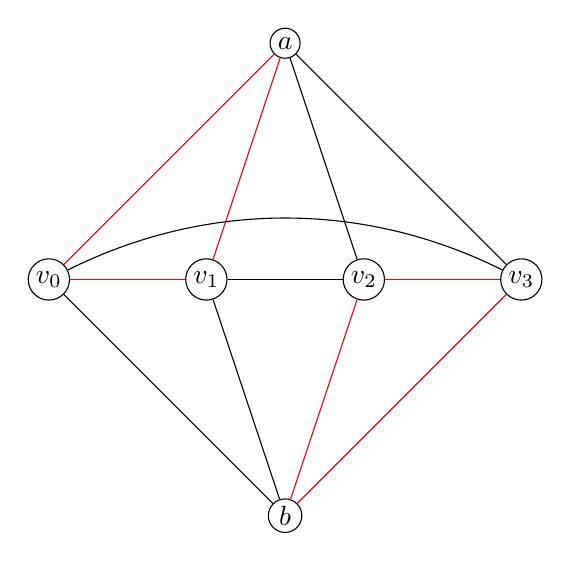
\begin{tikzpicture}[scale=1,every node/.style={draw,circle, inner sep=.05 cm}]
				%top and bottom vertices placed by hand
				\node (a) at (3,3){$a$};\node (b) at (3,-3){$b$}; 
				%%middle vertices drawn with a loop
				%% vertical edges drawn with a loop
				\foreach \i in {0,1,2,3}{
					\node  (\i) at (2*\i,0){$v_{\i}$};
					}
				%% draw straight edges around the middle
				\draw [color = red](a) -- (0);
				\draw [color = red](a) -- (1);
				\draw (a) -- (2);
				\draw (a) -- (3);
				\draw (0) -- (b);
				\draw [color = red](0)--(1);
				\draw (1) -- (b);
				\draw (1)--(2);
				\draw [color = red](2) -- (b);
				\draw [color = red](2)--(3);
				\draw [color = red](3)-- (b);
				\draw (0) .. controls (2,1) and (4,1) .. (3);

				\end{tikzpicture}
			\end{center}
		\end{proof}
		






		\end{enumerate}
	




	
\end{enumerate}

\end{document}


